\clearpage
\invisiblesection{Figures}
\begin{figure}[t!]
        \centering
        \caption[Adding weights to microphone and smartphone microphone]{The result of adding the determined weights on two signals: the microphone and a smartphone measurement.}
        
        \label{fig:weightson}
        \begin{subfigure}[t]{\textwidth}
			    \caption{Equalizing the mean of the gain of 40 microphone measurements.}
			    \label{fig:weightsonmic}
                \centering
    			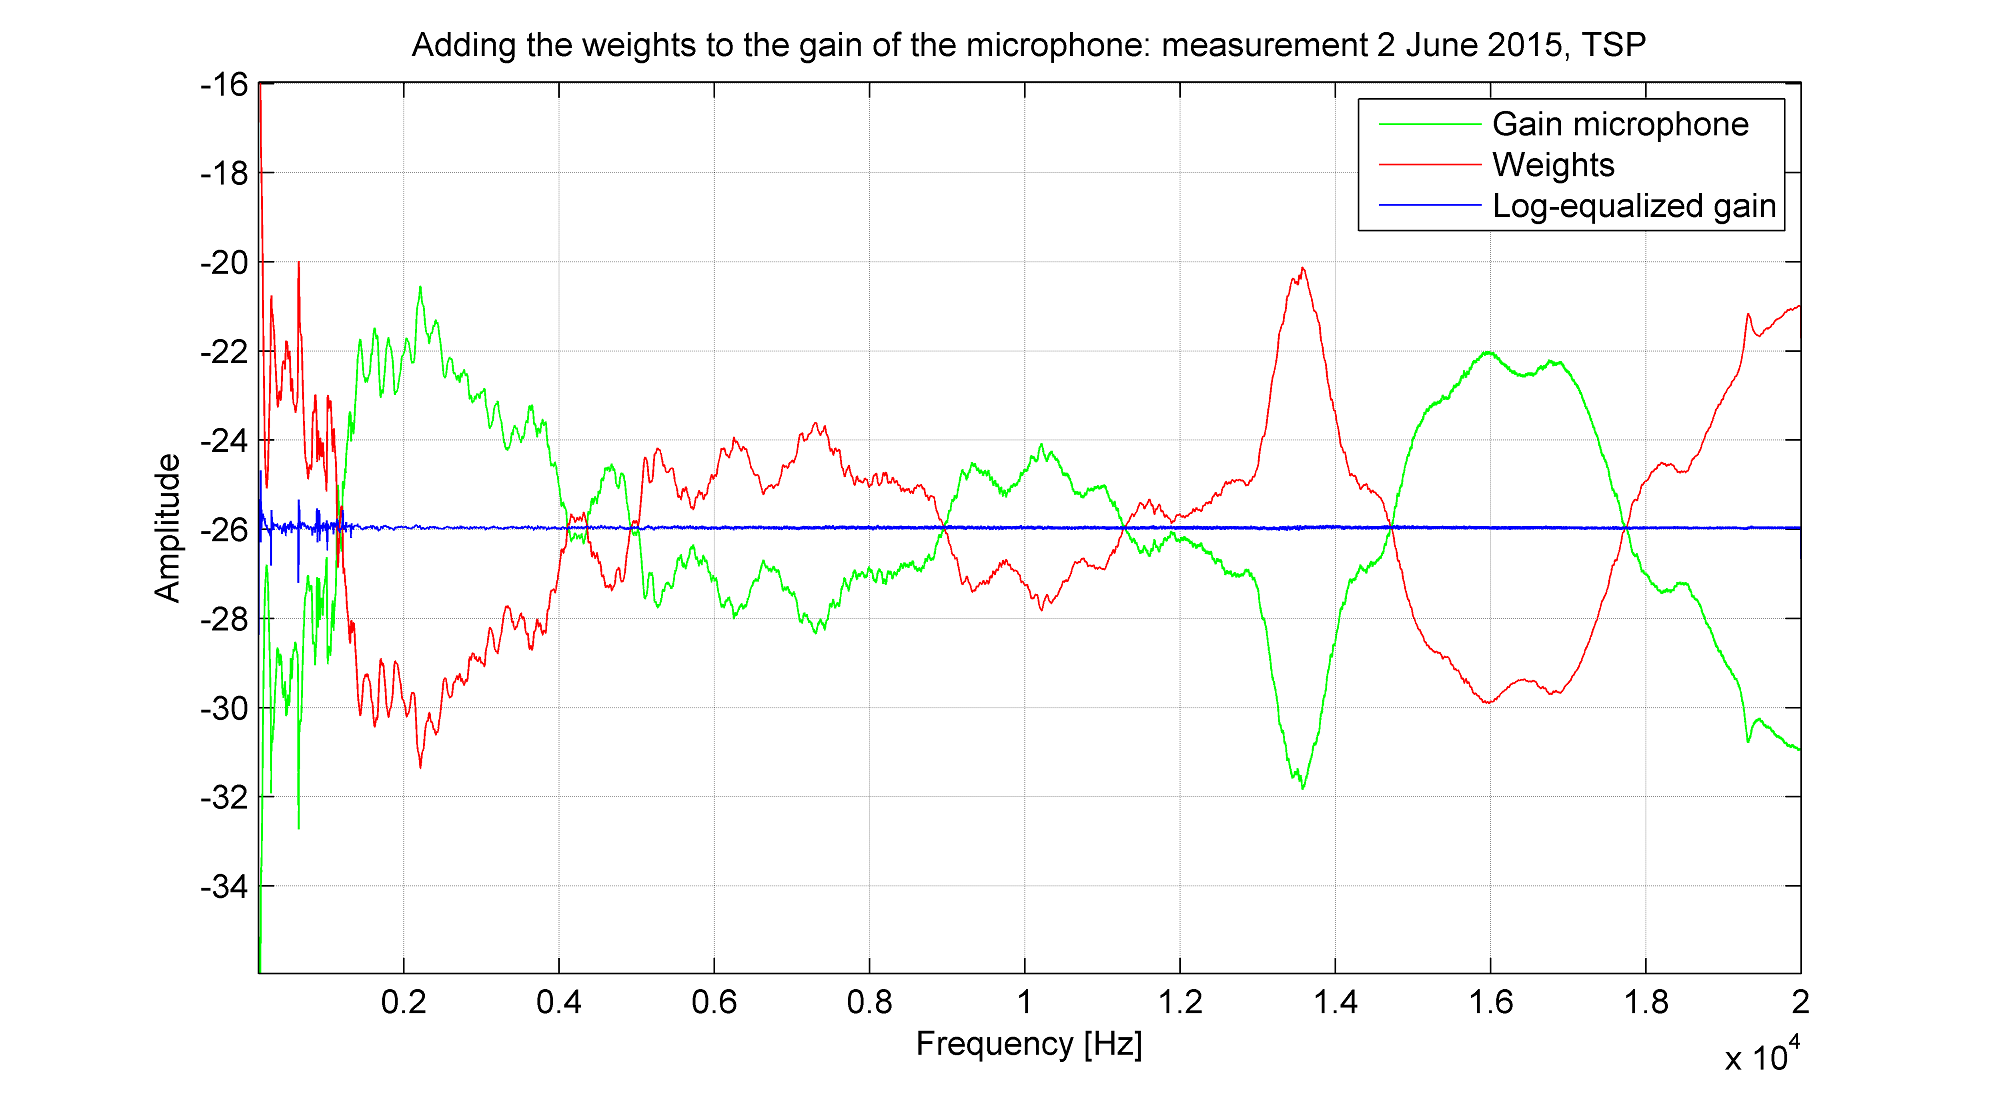
\includegraphics[width=\textwidth]{afbeeldingen/plots/weights-applied-microphone.png}
        \end{subfigure}%
        
        \begin{subfigure}[t]{\textwidth}
			    \caption{Equalizing the gain of {\nexus}, labelled with number 6, at $\phi=90^\circ$ and $\theta=0^\circ$}
			    \label{fig:weightsonphone}
                \centering
    			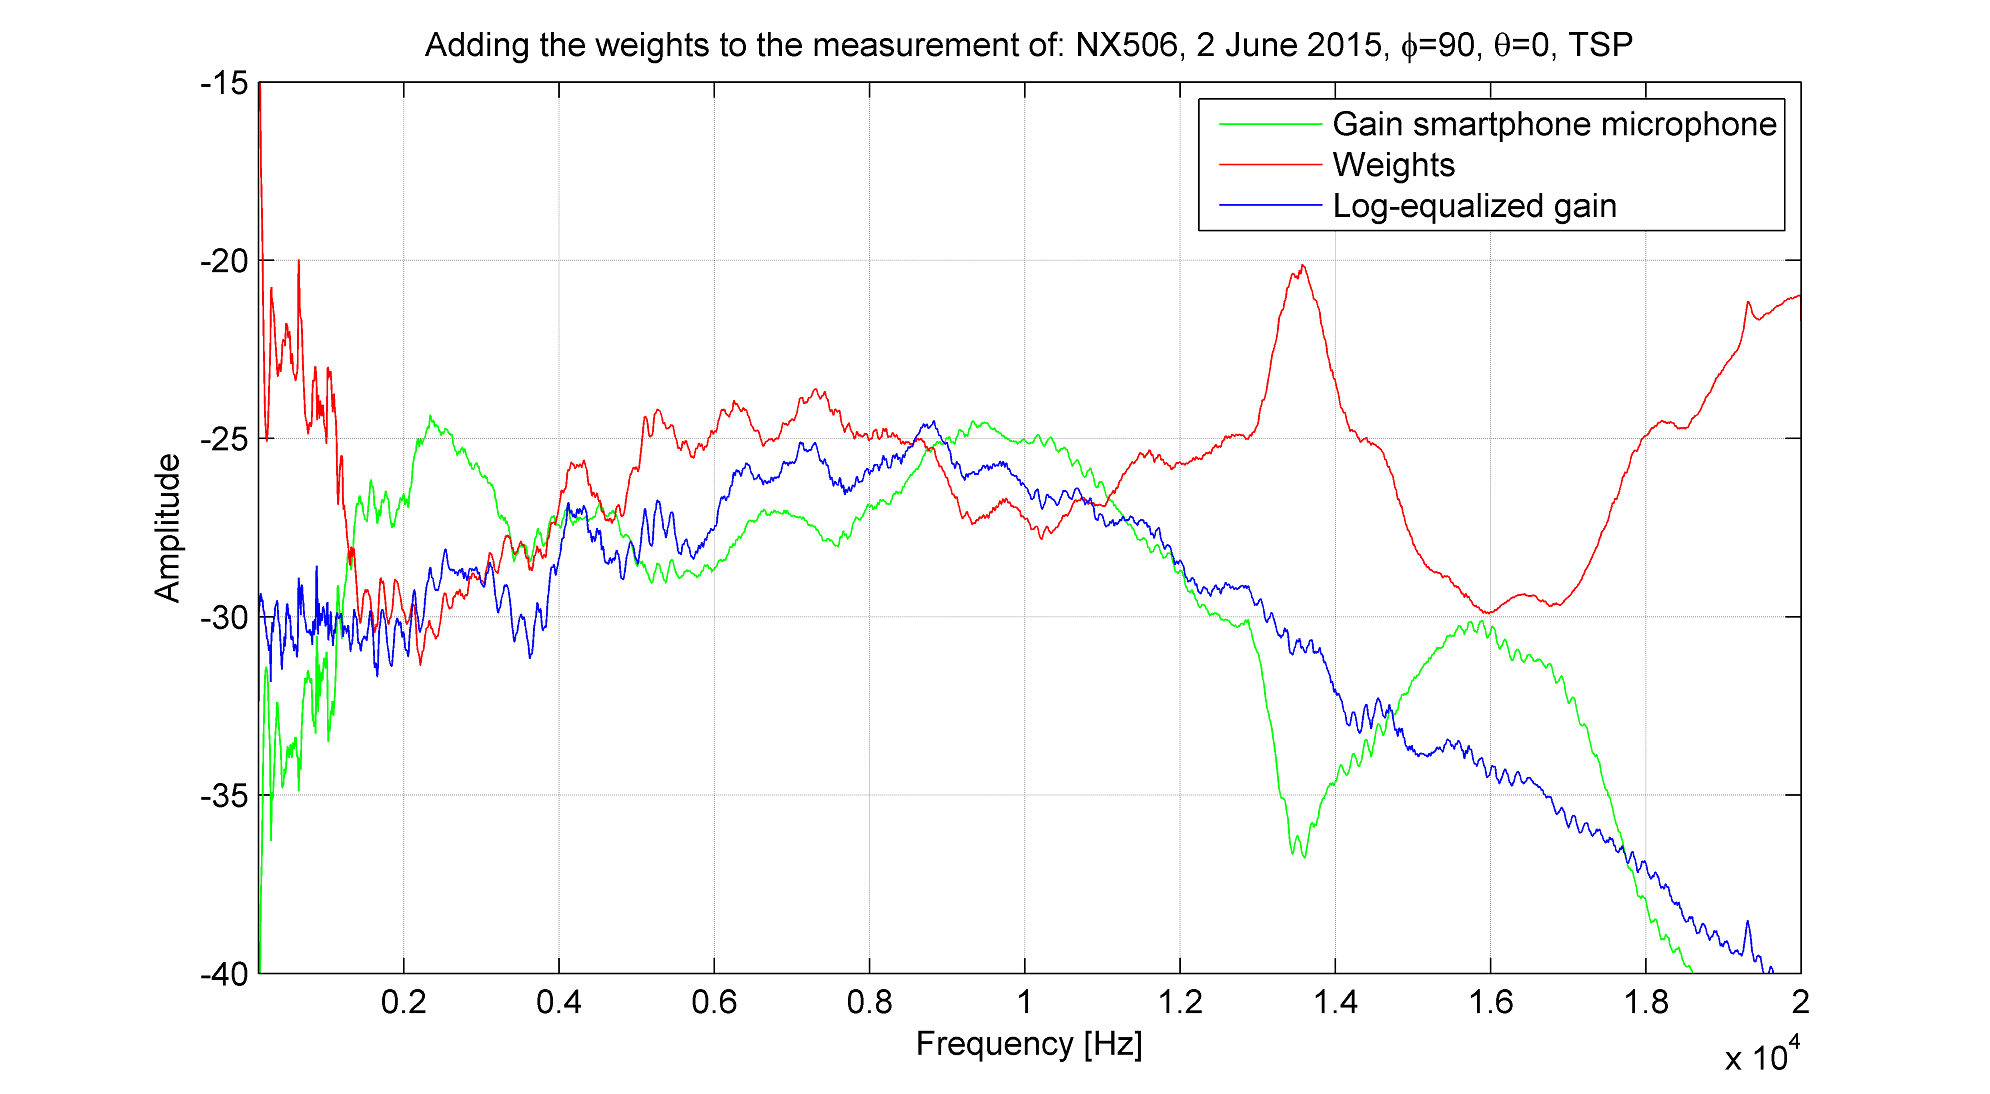
\includegraphics[width=\textwidth]{afbeeldingen/plots/weights-applied-smartphonemicrophone.png}
        \end{subfigure}
\end{figure}

\clearpage
\begin{figure}[t!]
        \centering
        \caption[Preliminary measurement results {\nexus} (6), equalized]{Preliminary measurement results of {\nexus}, labelled with number 6, at $\phi=90$ degrees, with limited frequency axis (from 125 Hz to 20 kHz) for the TSP measurement, non-equalized versus equalized.}
        \label{fig:06-eq-lin}
        \begin{subfigure}[t]{0.5\textwidth}
			    \caption{Non-equalized data on a linear frequency-scale}
			    \label{fig:before-eq-lin}
                \centering
    			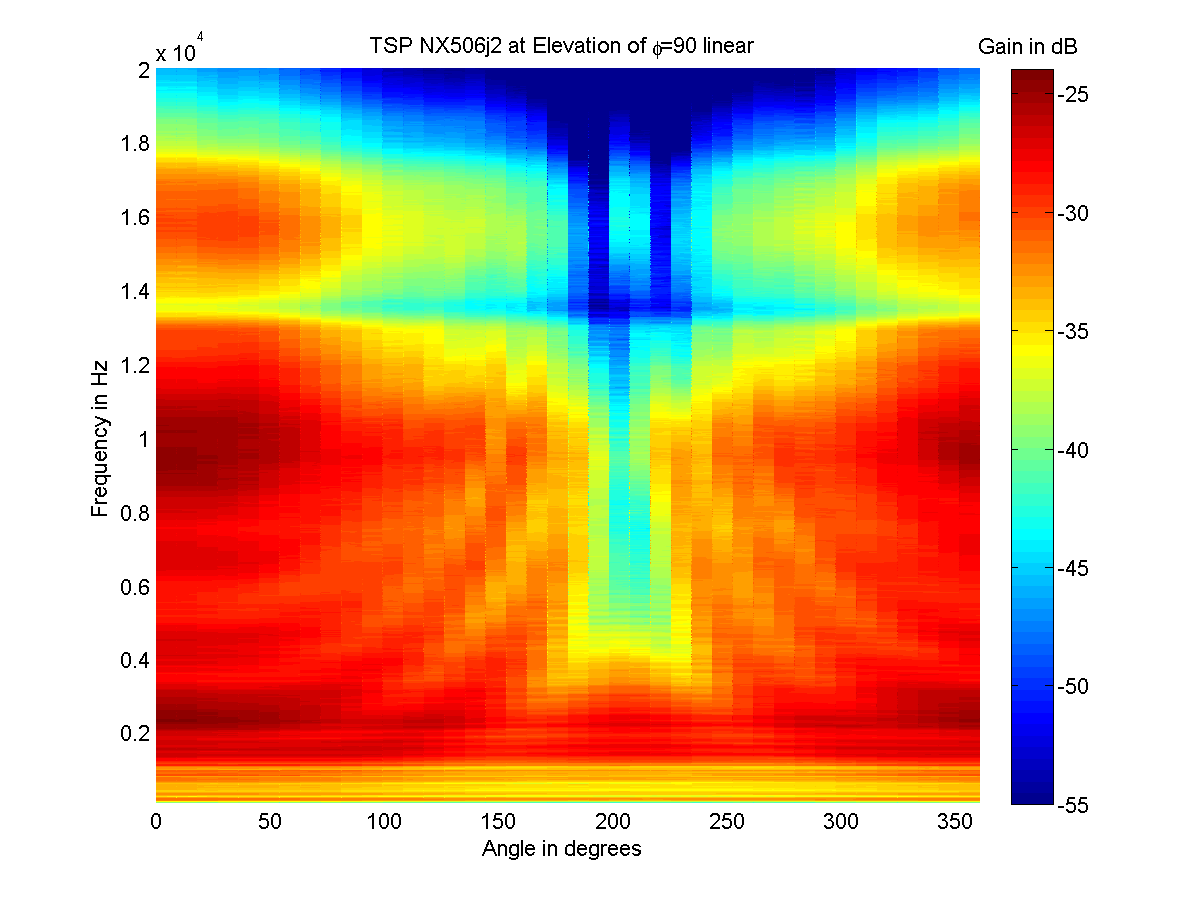
\includegraphics[width=\textwidth]{afbeeldingen/plots/NX506j2_TSP_090_lin.png}
        \end{subfigure}~
        \begin{subfigure}[t]{0.5\textwidth}
			    \caption{Equalized data on a linear frequency-scale}
			    \label{fig:after-eq-lin}
                \centering
    			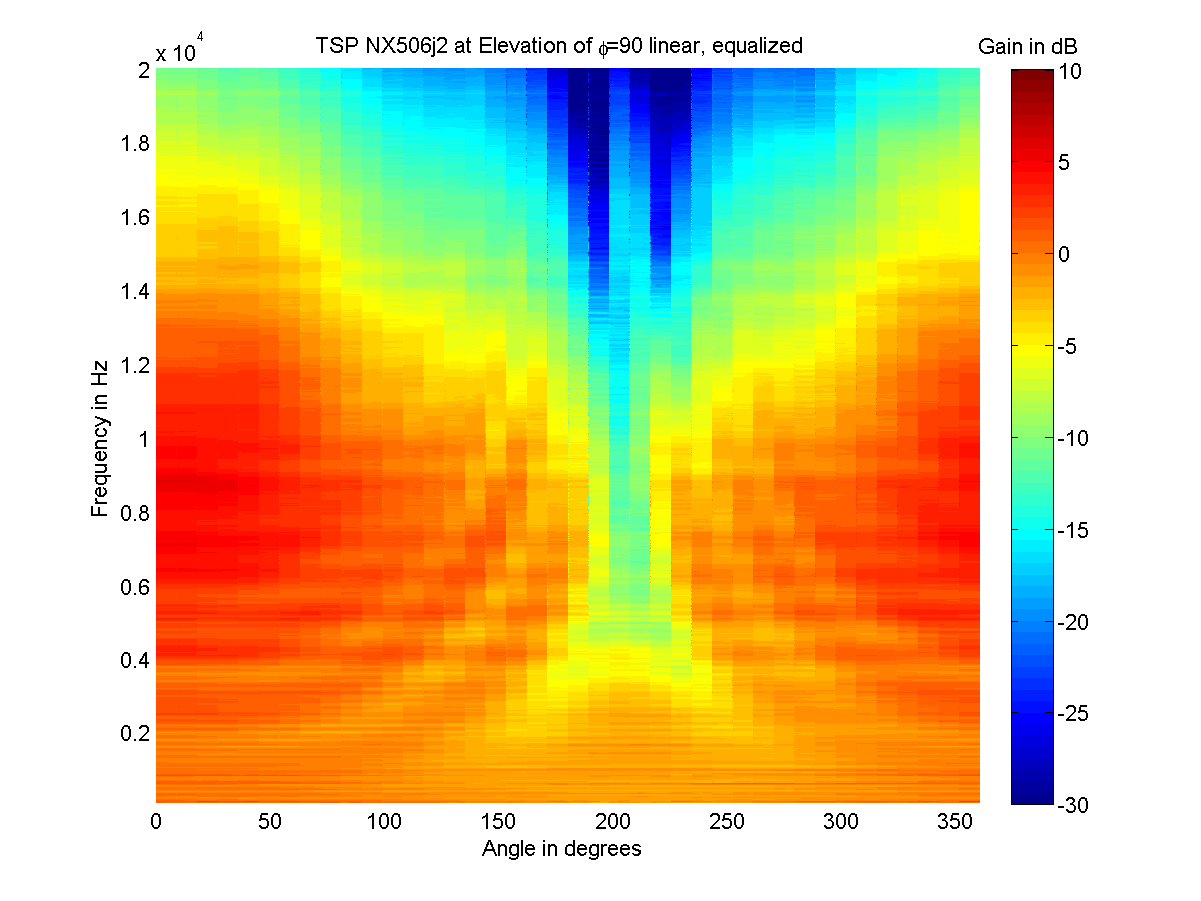
\includegraphics[width=\textwidth]{afbeeldingen/plots/NX506j2_TSP_090_lin_eq.png}
        \end{subfigure}
        
        \begin{subfigure}[t]{0.5\textwidth}
                \centering
			    \caption{Non-equalized data on a logarithmic frequency-scale}
			    \label{fig:before-eq-log}
    			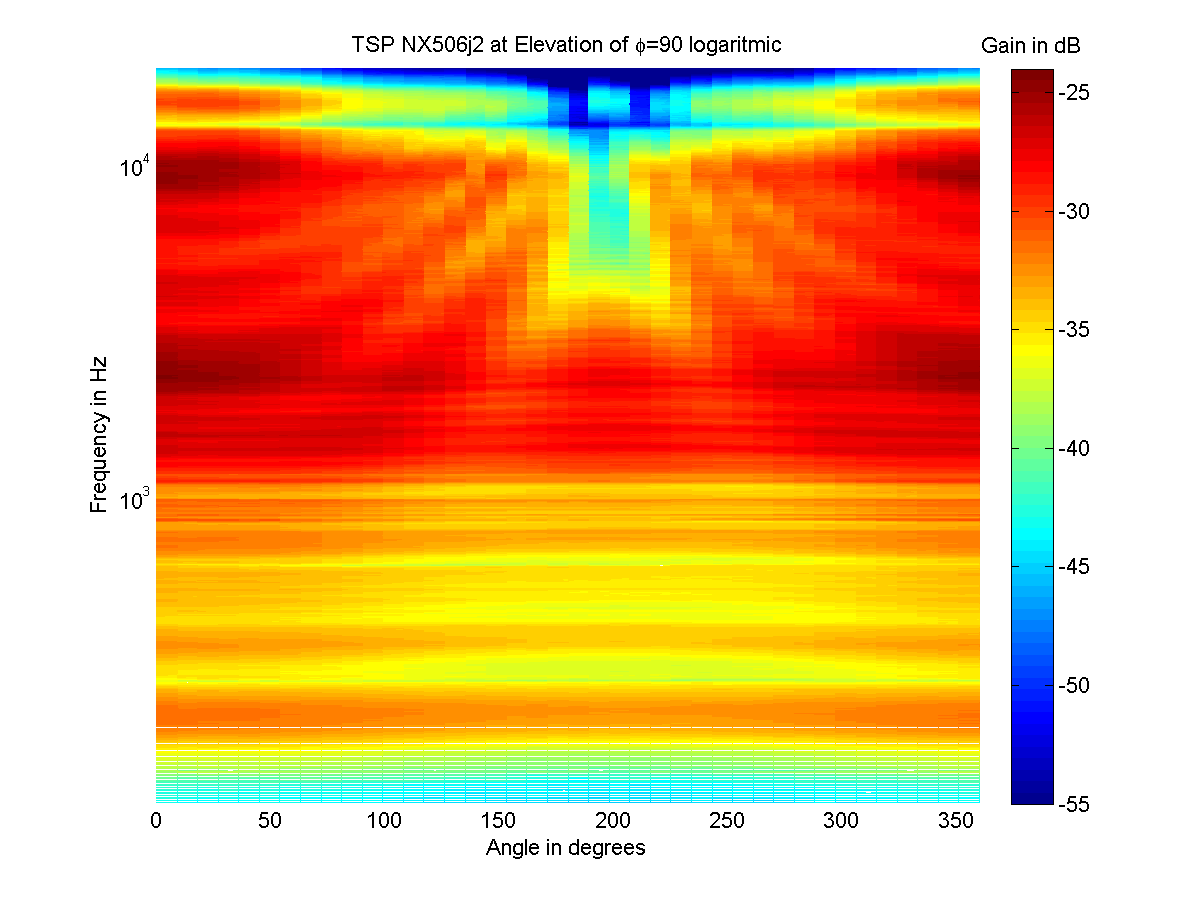
\includegraphics[width=\textwidth]{afbeeldingen/plots/NX506j2_TSP_090_log.png}
        \end{subfigure}~
        \begin{subfigure}[t]{0.5\textwidth}
                \centering
			    \caption{Equalized data on a logarithmic frequency-scale}
			    \label{fig:after-eq-log}
    			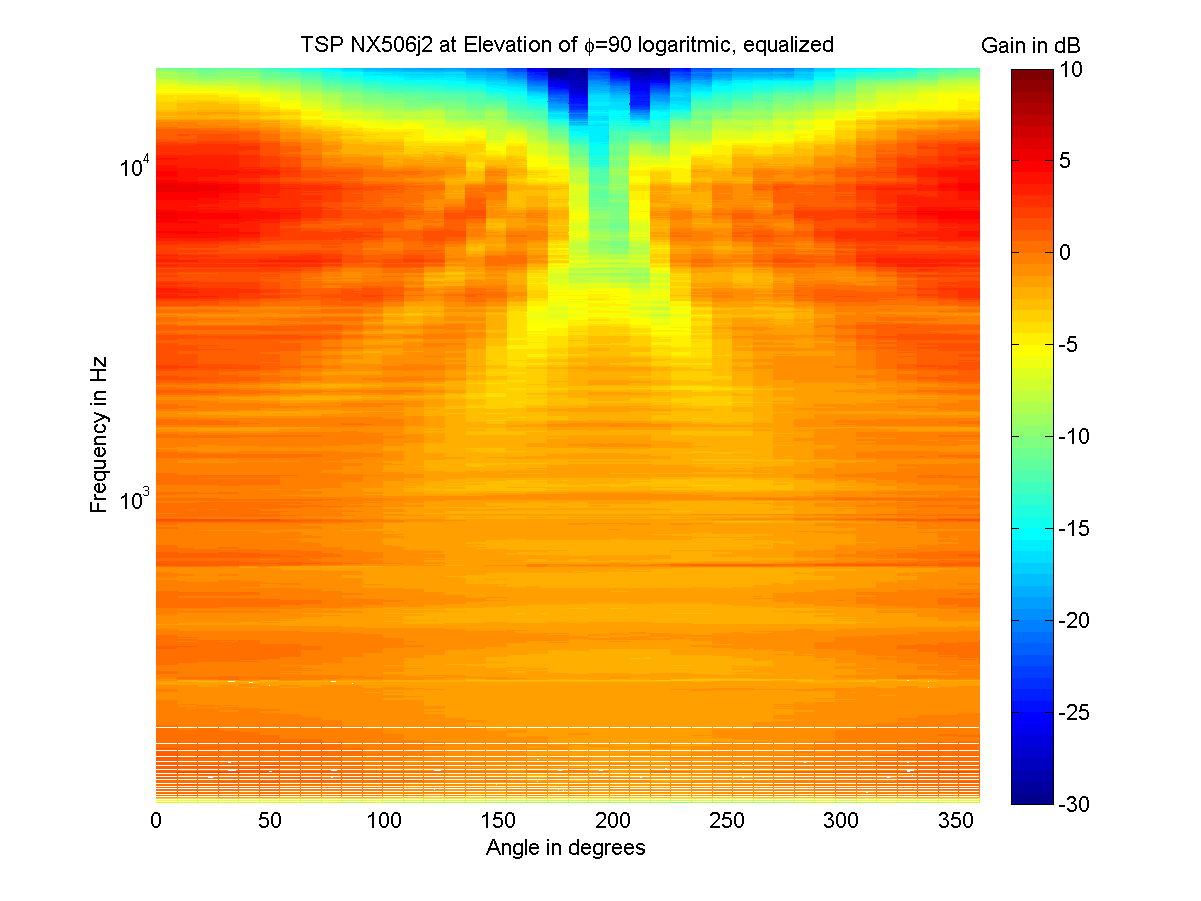
\includegraphics[width=\textwidth]{afbeeldingen/plots/NX506j2_TSP_090_log_eq.png}
        \end{subfigure}
\end{figure}